\documentclass[conference]{IEEEtran}

\usepackage{amsmath, amssymb}
\usepackage{graphicx}
\usepackage{cite}
\usepackage{url}
\usepackage{caption}
\usepackage{subcaption}
\usepackage{booktabs}
\usepackage{lipsum} % for lorem ipsum
\usepackage{algorithm}
\usepackage{algorithmic}
\usepackage{hyperref}
\usepackage[margin=1in]{geometry}
\usepackage{tabularx}
\usepackage{caption}
\usepackage{booktabs}
\usepackage{array} % Needed for new column type with borders
\usepackage{afterpage}


\title{Final Project Report 171}

\author{
\IEEEauthorblockN{
Laurel Jasper Murphy\IEEEauthorrefmark{1},
Gezheng Kang\IEEEauthorrefmark{2},
Ariana Smith\IEEEauthorrefmark{3},
Ayushi Kishore\IEEEauthorrefmark{4},
Varsha Sivaprakash\IEEEauthorrefmark{5}
}
\IEEEauthorblockA{\IEEEauthorrefmark{1}Dept. of Computer Science, UC Davis, Davis, CA, USA, ljamurphy@ucdavis.edu}
\IEEEauthorblockA{\IEEEauthorrefmark{2}Dept. of Computer Science and Engineering, UC Davis, Davis, CA, USA, gzkang@ucdavis.edu}
\IEEEauthorblockA{\IEEEauthorrefmark{3}Dept. of Computer Science, UC Davis, Davis, CA, USA, masmith@ucdavis.edu}
\IEEEauthorblockA{\IEEEauthorrefmark{4}Dept. of Computer Science, UC Davis, Davis, CA, USA, aykishore@ucdavis.edu}
\IEEEauthorblockA{\IEEEauthorrefmark{5}Dept. of Computer Science, UC Davis, Davis, CA, USA, varsivaprakash@ucdavis.edu}
}

\begin{document}
\maketitle

\begin{abstract}
This study uses data from the 2015 Behavioral Risk Factor Surveillance System (BRFSS) to develop a model that predicts diabetes status, categorized as no diabetes or diabetes. The target variable is based on self-reported medical diagnosis, excluding cases related solely to pregnancy. The dataset includes 21 predictive features capturing cardiovascular risk factors (e.g., high blood pressure, high cholesterol), behavioral indicators (e.g., smoking history, alcohol consumption, physical activity), demographic attributes (e.g., age, sex, education, household income), and general health conditions (e.g., obesity, sleep, and mental health). These features collectively provide a comprehensive overview of factors contributing to diabetes risk. We utilized and tested many models. 

We evaluated multiple models, including logistic regression, Bayesian networks, random forest, XGBoost, LightGBM, and several neural networks. Initial models achieved prediction accuracies ranging from 75\% to 88\%, but suffered from poor generalization due to suboptimal feature selection. After reworking the feature set and refining the model architecture, we saw all models improve to more then 90 percent accuracies. Then we scaled our neural network to an 11-layer architecture with 30 neurons per layer and ReLU activation. This final model achieved a test accuracy of 91.01\%. Although not the highest accuracy among all tested models, it exhibited the strongest generalization performance across evaluation metrics.
\end{abstract}

\vspace{0.5em}

\begin{IEEEkeywords}
diabetes prediction, Behavioral Risk Factor Surveillance System, machine learning, logistic regression, neural networks, public health
\end{IEEEkeywords}

\section{Introduction and Background}
Diabetes is a chronic metabolic disorder characterized by prolonged elevated blood glucose levels. This condition arises either from insufficient insulin production by the pancreas or the body's inability to effectively respond to insulin \cite{Roglic2016WHO}. The disease disrupts carbohydrate, fat, and protein metabolism and can lead to serious health complications, including cardiovascular disease, kidney failure, neuropathy, and vision loss. In the past few decades, diabetes has transformed from a rare disorder into a widespread public health crisis. The World Health Organization now classifies diabetes as one of the top ten causes of death worldwide, with projections indicating continuous growth in prevalence. \\

The human cost of diabetes is severe. Research indicates that individuals with diabetes are approximately 1.8 times more likely to die from any cause and over 2.3 times more likely to die from vascular disease compared to those without the condition. In terms of life expectancy, a person of 50 years with diabetes loses, on average, six years of life. The disease also increases susceptibility to various cancers, including those of the pancreas, liver, breast, and colon. The longer a person lives with undiagnosed or uncontrolled diabetes, the more likely they are to suffer irreversible health consequences.  \cite{Sarwar2010Diabetes} These facts underscore the critical importance of early detection and proactive management. \\

From an economic perspective, the burden is equally significant. According to estimates, the global cost of diabetes surpasses USD 1.3 trillion annually, accounting for nearly 1.8 percent of the global GDP. These expenses encompass both direct healthcare costs (such as hospitalizations, medications, and physician visits) and indirect costs (including lost productivity, premature mortality, and long-term disability). Particularly in low and middle income countries, where healthcare access is limited, the indirect costs are disproportionately high, leading to further socioeconomic disparities in outcomes. \cite{Bommer2017Global} Without significant improvements in prevention, early screening, and chronic disease management, these costs are expected to escalate dramatically in the coming decades. \\

To address the growing crisis of the diabetes pandemic, new technologies must be explored to assist with early detection and intervention. One of the most promising frontiers is artificial intelligence (AI) and machine learning (ML), which can process complex, high-dimensional datasets and identify subtle patterns that traditional methods may overlook. These technologies offer the potential to provide inexpensive, scalable, and non-invasive diagnostic support, particularly in underserved areas where medical personnel or equipment may be scarce. \\

This project examines the intersection of AI and healthcare by developing a predictive model for diabetes risk. Using data from the CDC’s Behavioral Risk Factor Surveillance System (BRFSS), we leverage a cleaned and balanced version of the Diabetes Health Indicators dataset. This dataset comprises 21 behavioral and demographic features, including physical health, diet, body mass index (BMI), education, income, and access to healthcare services. Rather than treating diabetes as a three-class problem (type 0, 1, or 2), we simplified the task into a binary classification—predicting whether an individual does or does not have diabetes. \\

Our motivation for choosing this topic stems from both the scale of the public health crisis and the opportunity to create a meaningful, real-world application of AI. Early diagnosis of diabetes has been shown to reduce complications and improve quality of life significantly. However, current screening methods are often reactive rather than proactive, missing opportunities to identify individuals at risk before symptoms manifest. By building a machine learning model trained on behavioral and self-reported data, we aim to develop a method for early detection that can be deployed in mobile applications, telehealth platforms, or community screening initiatives.
We tested several modeling approaches, including logistic regression and Bayesian classifiers, but ultimately focused on designing a deep learning model: a six-layer artificial neural network. This network was optimized through grid search, hyperparameter tuning, and extensive evaluation, achieving around 91 percent accuracy on held-out data. While this accuracy reflects room for improvement, our research highlights the feasibility of developing an AI-powered screening tool that strikes a balance between precision, recall, and interpretability. \\

This work contributes to a growing body of research on AI in healthcare. It demonstrates how predictive models can be trained on accessible datasets to assist in early disease detection. In the future, such models could be integrated into broader preventive healthcare strategies, serving as early warning systems that alert individuals and healthcare providers to elevated risk—before disease progression. \\

\section{Literature Review}
Recent literature emphasizes the importance of selecting appropriate modeling techniques and preprocessing strategies for health-related classification tasks. Traditional models like binomial logistic regression remain effective for categorical datasets, particularly when regularization and optimal feature selection are applied, as shown by high accuracy and low AIC scores. Neural networks, on the other hand, are well-suited to capturing complex, non-linear patterns in one-hot encoded categorical data, with architectures benefiting from techniques such as L1/L2 regularization, ReLU activation, and hyperparameter tuning via tools like KerasTuner. Overall, such approaches demonstrate the evolving landscape of machine learning in medical diagnostics, where model performance hinges on careful data transformation, architecture design, and context-specific evaluation metrics.\\

A robust body of research supports the inclusion of the 21 features in our diabetes prediction model. Clinical studies confirm that high blood pressure, BMI, and smoking are strong predictors of diabetes due to their links with insulin resistance and inflammation ( \cite{lambert2021hypertension}; \cite{yashi2023obesity}; \cite{li2014fruitveg}). Dietary habits, such as low fruit and vegetable intake, also correlate with increased diabetes risk, while regular physical activity offers protective benefits \cite{sun2013fruit}; \cite{song2008fruit}; \cite{williams2008exercise}). Cholesterol levels and regular cholesterol checks are relevant due to evidence of low HDL in some diabetes subtypes (\cite{kennedy1978hdl}). Mental health and general health status are important, as diabetes often coexists with depression and chronic illness (\cite{gornik2010hyperglycaemia}). Socioeconomic factors—including income, education, insurance status, and healthcare access—influence diagnosis and management, particularly in underserved communities (\cite{zhu2012insurance}; \cite{patzer2021access}; \cite{lysy2013income};\cite{choi2024education}). Cost-related barriers often delay care, worsening outcomes (IHPI). Demographics like age and sex affect susceptibility, with older adults and postmenopausal women at higher risk (\cite{moore2003age}; \cite{gale2001rise}). Finally, difficulty walking is linked to diabetes-related neuropathy and vascular dysfunction (\cite{brach2008gait}). Together, these features enhance the accuracy and real-world applicability of our predictive model.

\section{Dataset Description and Exploratory Data Analysis}
Dataset description:
The dataset we used was the Diabetes Health Indicators from the CDC.  This dataset consisted of 3 classes of diabetes and 21 features.  0 indicated no diabetes, 1 indicated type 1 diabetes and 2 indicated type 2 diabetes.  We treated this problem as a binary classification task, where the predictions indicate whether or not a person has diabetes based on a given set of features.  Upon observing the distribution of the features and diabetes classes, we quickly realized that there was a huge class imbalance between positive and negative cases of diabetes, with over 80 percent of the dataset having no diabetes. \\ 
To mitigate this imbalance, we found the same dataset, but with negative diabetes cases randomly dropped.  Here, the negative cases were indicated by 0 and positives were indicated by 1, while still having 21 features.  Some of the features were continuous values, while most were categorical values.  Below are the features:\\

\begin{itemize}
  \item \textbf{Continuous:} MentHlth, PhyHlth, BMI
  \item \textbf{Discrete:} HighBP, HighChol, CholCheck, Smoker, Stroke, HeartDiseaseorAttack, PhysActivity, Fruits, Veggies, HvyAlcoholConsump, AnyHealthcare, NoDocbcCost, GenHlth, DiffWalk, Sex, Age, Education, Income
  \item \textbf{Target (Discrete 0 or 1):} \texttt{Diabetes\_binary}
\end{itemize}

\vspace{1em}

\noindent
\textbf{Exploratory Data Analysis}:

Before any data cleaning, all model accuracies were roughly around 75%. 
We computed the linear correlation using pearson correlation between continuous and continuous pairs and point-biserial correlation between categorical and continuous pairs.  Based on these computations, none of the feature pairs had strong linear correlation.  
The first attempt of cleaning involved outlier detection and removal.  Using the interquartile range method, we were able to detect outliers for all continuous variables: BMI, Mental Health and Physical Health.  We decided to remove these outliers to avoid the skewed data from disrupting our model performances.  However, we noticed how the data points were almost halved upon removing the outliers, indicating that the outliers must be significant to the model’s predictions. 

Next, we conducted a literature review for all 21 features which confirmed the correlation of all features with diabetes, including the continuous features for which the outliers were removed.  

To reduce the effects of the skewed distribution of the continuous variables, we decided to categorize them into 4-5 classes each based on their value ranges.  This change was the key part of our EDA, after which the model accuracies significantly improved, going upto around 90 percent.  Upon further plotting, the data was significantly less skewed compared to pre-categorization.

Finally, on our now fully categorical dataset, we decided to identify the most important features using the Chi-Squared coefficient which is used for detecting non-linear dependencies between categorical variables. Based on this, the following features were selected as the most important:  

\begin{itemize}
  \item \texttt{HighBP}
  \item \texttt{HighChol}
  \item \texttt{NEW\_BMI\_class}
  \item \texttt{Stroke}
  \item \texttt{HeartDiseaseorAttack}
  \item \texttt{PhysActivity}
  \item \texttt{HvyAlcoholConsump}
  \item \texttt{GenHlth}
  \item \texttt{MetHlth\_Class}
  \item \texttt{PhyHlth\_Class}
  \item \texttt{DiffWalk}
  \item \texttt{Age}
  \item \texttt{Income}
\end{itemize}
\vspace{1em}

However, most model performances decreased slightly overall when any of the features were removed, indicating that all features carried some importance towards the prediction of diabetes, as supported by our feature literature review.  Therefore, we kept all 21 features most of the time during our study unless necessary to remove, since all features have some significance to the prediction of diabetes.\\


\section{Proposed Methodology}
All features in this dataset are categorical, meaning they represent qualitative labels, not numerical quantities. Therefore, standardization is not appropriate. For instance, the HighBP feature uses 0 to indicate no high blood pressure and 1 to indicate presence of high blood pressure. Standardizing this would incorrectly imply that 1 > 0 in a numerical sense, which distorts the categorical nature of the data. To handle categorical features correctly, we applied one-hot encoding, which converts values like 0 and 1 into distinct vectors such as [1, 0] and [0, 1].\\ 

In addition, we bucketed the continuous features BMI, MentHlth, and PhysHlth into discrete classes based on meaningful thresholds. For example, BMI is categorized into five classes (0 through 4). More details on the binning criteria can be found in the final text cell of the notebook. Since artificial neural networks (ANNs) are capable of capturing both linear and non-linear relationships, we fed the entire encoded dataset into the model without additional feature engineering.\\

The model consists of 11 total layers: 1 input layer, 10 hidden layers, and 1 output layer. Each hidden layer contains 30 neurons and uses the ReLU activation function. The output layer uses a sigmoid activation function, suitable for binary classification. L1 and L2 regularization (each set to 0.001) was applied across all layers to reduce overfitting. The SGD optimizer was used with a momentum of 0.9 to accelerate convergence. The ANN achieved high accuracy on the test set, indicating good generalization. The confusion matrix and derived metrics (precision, recall, F1-score) also showed strong performance, confirming that the model effectively captured the relationship between the features and the target variable. The ANN model performed well with the fully one-hot encoded dataset, validating that proper encoding and a well-structured neural network can effectively model complex relationships in categorical health-related data.\\

To better understand the learning behavior of **ANN Model A**, we visualized the model’s training dynamics over 100 epochs.\\

\begin{figure}[H]
  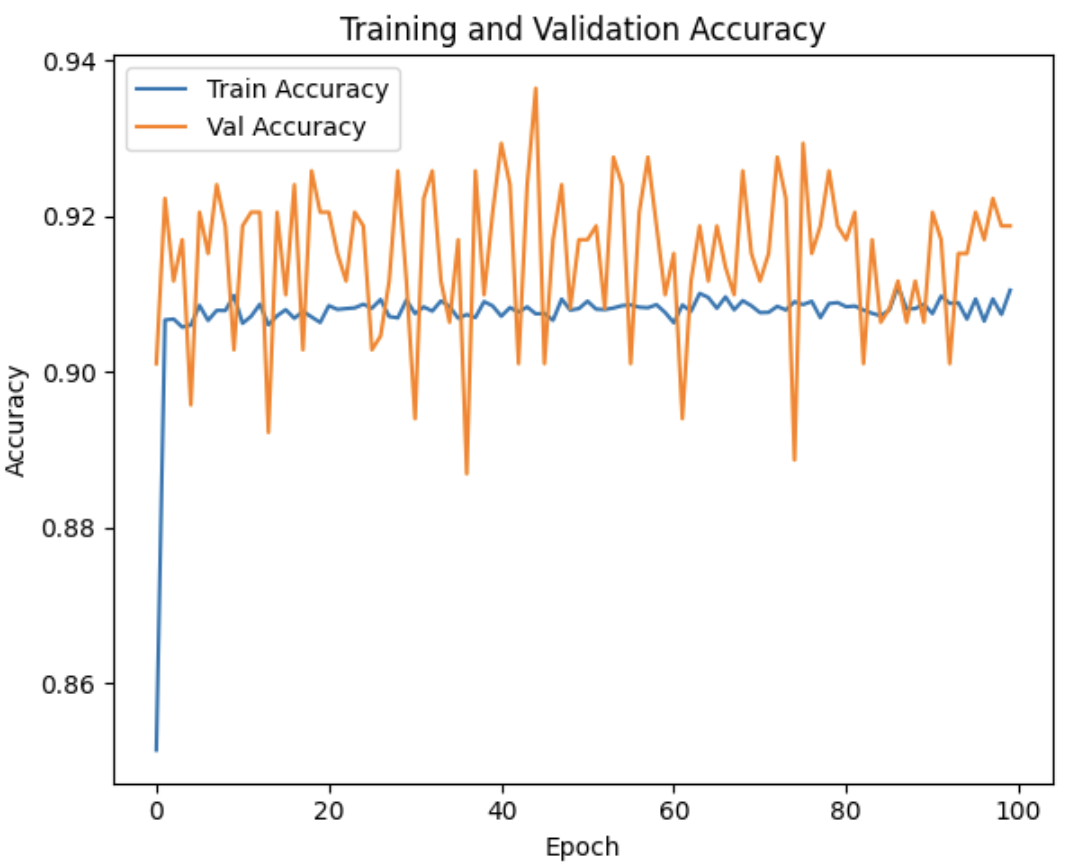
\includegraphics[width=0.5\textwidth]{training_accuracy_ANN_A.png} % change filename & width as needed
  \caption {shows a smooth convergence trend, with both training and validation loss decreasing steadily. Slight overfitting is observed in later epochs, but regularization mitigates major divergence.}
  \label{fig:my_label}
\end{figure}

\begin{figure}[H]
  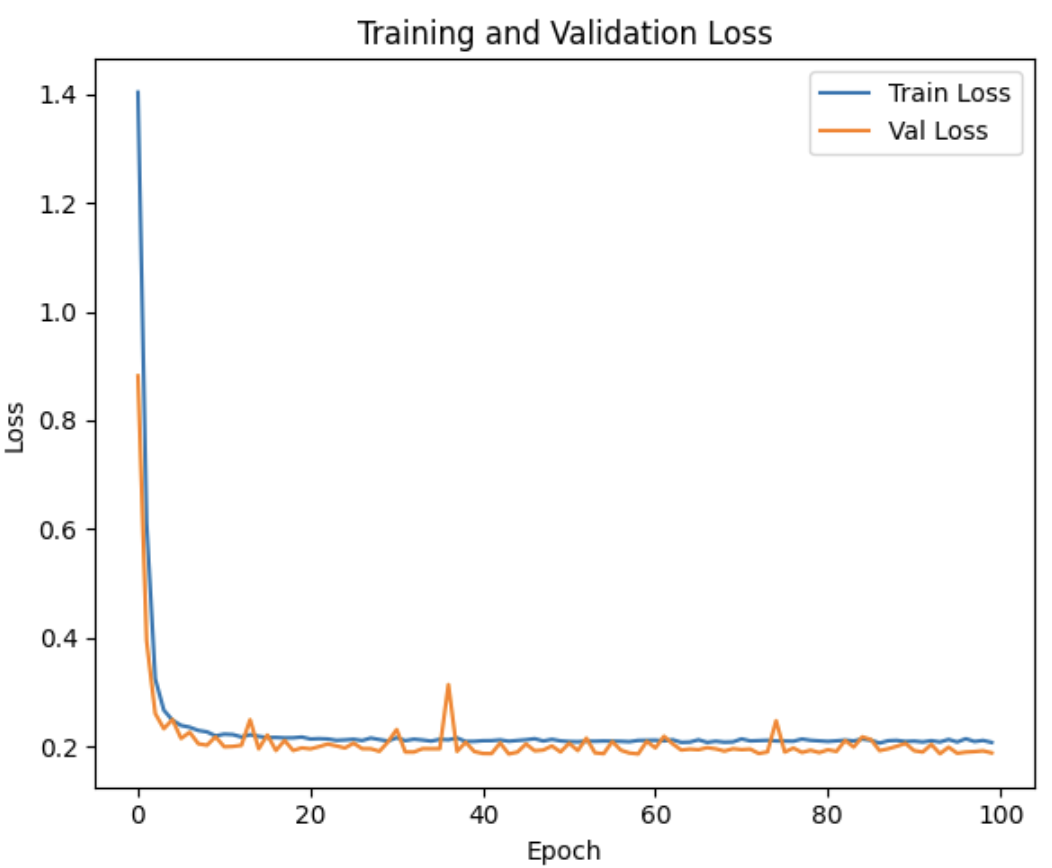
\includegraphics[width=0.5\textwidth]{training_loss_ANN_A.png} % change filename & width as needed
  \caption {Indicates consistent accuracy growth for both training and validation sets. The final accuracy plateau suggests successful training convergence.}
  \label{fig:my_label}
\end{figure}
\\

These trends confirm the model’s learning capacity and generalization ability, though fine-tuning can further improve its performance and reduce training time.\\

\section{Experimental Results and Evaluation}
This section presents the results of our comparative evaluation of different classification models, including Logistic Regression, several Artificial Neural Network (ANN) architectures, Bayesian Network, and Tree-based models like Random Forest, XGBoost, and LightGBM. Each model was evaluated using consistent metrics: confusion matrix, accuracy, precision, recall, F1 score, and testing time.\\

\noindent
\textbf{Model 1) Binomial logistic regression}:\\
Binomial logistic regression was applied to a fully categorical dataset (3 to classes) with no need for standardization, binary class labels, and equal class weighting. No outliers were removed prior to modeling. The same optimization techniques as in previous models were used, and four models were tested in total. The best-performing models (a and b) used all 21 features, with Model a employing L2 regularization and the 'lbfgs' solver. Model a achieved the highest accuracy (91.06 percent) and a low AIC (5123.826), while Model b had a nearly identical classification report with a slightly lower AIC (5113.101). Models c and d, which used only 13 features, matched Model a’s accuracy but had higher AIC scores and the highest number of false negatives (753), a critical factor in medical data contexts. These results indicate that including all 21 features was necessary for optimal classification performance.\\

\noindent
\textbf{Model 2) ANN B:}:\\
After exploratory data analysis, we implemented a binary classifier for diabetes risk. We split the data 80-20 into train and test sets, and constructed a six-layer feedforward Artificial Neural Network with Tensorflow/Keras. The hidden layers utilized the ReLU activation function, and we tried different L1 and L2 regularization weights to prevent overfitting of the model. The output layer uses the default sigmoid function and binary cross-entropy loss to improve the binary classifier. We implemented a brute-force grid search with five hyperparameters to hyperparameter tune the ANN, an SGD learning rate and momentum, a hidden layer with either 16 or 32 neurons, and L1/L2 regularization. We also ran this over 50 epochs and a batch size of 64.
This brute force grid search method generalized our six-layer network’s hyperparameters and provided a reproducible model from the root BRFSS features to a tuned diabetes‐risk predictor.\\ 

\noindent
\textbf{Model 4) ANN C and KerasTuner}:\\
Implemented a supervised machine learning pipeline to predict diabetes using a feedforward neural network with hyperparameter tuning. The process begins with loading and preprocessing a dataset, where the target variable is extracted and categorical features are one-hot encoded. The data is then split into training and testing sets, followed by standardization using StandardScalar. A custom model-building function is defined using KerasTuner, allowing for dynamic architecture adjustments, including varying the number of layers, units per layer, and learning rate. A RandomSearch tuner is employed to identify the best model configuration by optimizing for validation accuracy. Early stopping is incorporated to prevent overfitting. The best model is re-trained and evaluated on the test set, reporting both accuracy and optimal hyperparameters. Finally, the training history, confusion matrix, and other parameters are visualized to show trends in loss and accuracy over epochs, providing insight into the model's learning behavior and results.\\

\noindent
\textbf{Model 5) Random Forest}:\\
We implemented Random Forest using the RandomForestClassifier from scikit-learn. All features were one-hot encoded to handle categorical variables properly. To address the class imbalance in the target variable, we used class\_weight='balanced', which automatically adjusts the weight inversely proportional to class frequencies. The model was trained and validated using 5-fold stratified cross-validation, and performance was evaluated using accuracy, precision, recall, F1 score, and testing time. Finally, the model was retrained on the full training set and tested on the held-out test set to assess generalization.\\

\noindent
\textbf{Model 6) XGBoost}:\\
The XGBoost model was implemented using XGBClassifier. We configured the objective as 'binary\:logistic' for binary classification and used 'logloss' as the evaluation metric. The tree\_method='hist' was selected for faster training on structured data. Because XGBoost does not natively support class\_weight, we manually computed sample weights based on the class distribution and passed them during model fitting. Similar to Random Forest, we performed 5-fold stratified cross-validation to evaluate the model, followed by a final evaluation on the test set. The model's robustness and fast inference make it attractive for structured medical data.\\

\noindent
\textbf{Model 7) LightGBM}:\\
We used the LGBMClassifier to implement the LightGBM model, setting the objective to 'binary'. The parameter class\_weight='balanced' ensured that the model addressed class imbalance effectively. We used 100 estimators and a fixed random\_state=42 for reproducibility. LightGBM’s ability to handle large numbers of features and fast inference made it particularly suitable for our one-hot encoded dataset. As with the other models, evaluation was conducted through 5-fold cross-validation, followed by a final test set evaluation to confirm model performance and generalization.

\vspace{1em}

\textbf{Models and Hyperparameters}:

\begin{table}[htbp]
  \centering
  \renewcommand{\arraystretch}{1.3}
  \begin{tabular}{|p{3.5cm}|p{3cm}|}
    \hline
    \textbf{Model} & \textbf{Key Hyperparameters} \\
    \hline
    Logistic Regression (L2) & Solver: 'lbfgs', Penalty: 'L2', C = 1.0, AIC = 5123.826 \\
    \hline
    Logistic Regression (L1) & Solver: 'liblinear', Penalty: 'L1', C = 1.0, AIC = 5113.101 \\
    \hline
    ANN Model A & 10 layers with 30 neurons/layer, Activation: ReLU, Sigmoid output, Regularization: L1L2(0.001), SGD+momentum(0.9), LR=0.01, Epochs=100, Batch=64, Loss: binary\_crossentropy \\
    \hline
    ANN Model B & 6 layers, 16 neurons/layer, Activation: ReLU, Sigmoid output, Regularization: L1L2(0.0), SGD+momentum(0.9), LR=0.01, Epochs=50, Batch=64, Loss: binary\_crossentropy \\
    \hline
    ANN C (Tuned) & Layers: [128, 64, 64, 16, 128, 64], ReLU + Sigmoid, Optimizer: Adam, LR=0.0062, Epochs=30, Batch=64 \\
    \hline
    Bayesian Network & HillClimbSearch, Scoring: K2, Inference: Variable Elimination \\
    \hline
    Random Forest & class\_weight='balanced', random\_state=42 \\
    \hline
    XGBoost & objective='binary:logistic', eval\_metric='logloss', tree\_method='hist', random\_state=42 \\
    \hline
    LightGBM & objective='binary', class\_weight='balanced', n\_estimators=100, random\_state=42 \\
    \hline
  \end{tabular}
  \caption{Models and their key hyperparameters used in evaluation and analysis.}
  \label{tab:model_params}
\end{table}

% \noindent
% \textbf{Overall Performance Metrics:}
% \vspace{0.5em}

% \begin{table*}[htbp]
% \centering
% \renewcommand{\arraystretch}{1.3}
% \begin{tabular}{|p{4.5cm}|c|c|c|c|c|}
% \hline
% \textbf{Model} & \textbf{Accuracy} & \textbf{Precision} & \textbf{Recall} & \textbf{F1 Score} & \textbf{Testing Time (s)} \\
% \hline
% \rule{0pt}{2.5ex}Logistic Regression A (L2 - lbfgs) & 0.9100 & 0.9100 & 0.9100 & 0.9100 & $<0.003$ \\
% \hline
% \rule{0pt}{2.5ex}Logistic Regression B (L1 - liblinear) & 0.9100 & 0.9100 & 0.9100 & 0.9100 & $<0.003$ \\
% \hline
% \rule{0pt}{2.5ex}Bayesian Network (BN) & 0.9100 & 0.9100 & 0.9100 & 0.9100 & 7.754 \\
% \hline
% \rule{0pt}{2.5ex}ANN Model A & 0.9107 & 0.9213 & 0.9111 & 0.9027 & 9.714 \\
% \hline
% \rule{0pt}{2.5ex}ANN Model B & 0.9098 & 0.9031 & 0.9180 & 0.9105 & 9.524 \\
% \hline
% \rule{0pt}{2.5ex}ANN Grid-Tuned (Best Trial) & 0.9087 & 0.9261 & 0.9104 & 0.9073 & 9.298 \\
% \hline
% \rule{0pt}{2.5ex}Random Forest & 0.8980 & 0.8977 & 0.8982 & 0.8981 & 3.6610 \\
% \hline
% \rule{0pt}{2.5ex}XGBoost & 0.9047 & 0.9054 & 0.9047 & 0.9047 & 1.6345 \\
% \hline
% \rule{0pt}{2.5ex}LightGBM & 0.9067 & 0.9072 & 0.9067 & 0.9067 & 0.6305 \\
% \hline
% \end{tabular}
% \caption{Evaluation metrics and testing time for each model.}
% \label{tab:performance_metrics}
% \end{table*}

\begin{table}[H]
\centering
\caption{Evaluation metrics and testing time for each model.}
\label{tab:performance_metrics}
\renewcommand{\arraystretch}{1.2}
\begin{tabular}{|l|c|c|c|c|c|}
\hline
\textbf{Model} & \textbf{Acc.} & \textbf{Prec.} & \textbf{Rec.} & \textbf{F1} & \textbf{Time (s)} \\
\hline
LogReg (L2) & 0.9100 & 0.9100 & 0.9100 & 0.9100 & $<$0.003 \\
LogReg (L1) & 0.9100 & 0.9100 & 0.9100 & 0.9100 & $<$0.003 \\
BN          & 0.9100 & 0.9100 & 0.9100 & 0.9100 & 7.754 \\
ANN A       & 0.9107 & 0.9213 & 0.9111 & 0.9027 & 9.714 \\
ANN B       & 0.9098 & 0.9031 & 0.9180 & 0.9105 & 9.524 \\
ANN Tuned   & 0.9087 & 0.9261 & 0.9104 & 0.9073 & 9.298 \\
RF          & 0.8980 & 0.8977 & 0.8982 & 0.8981 & 3.661 \\
XGB         & 0.9047 & 0.9054 & 0.9047 & 0.9047 & 1.634 \\
LGBM        & 0.9067 & 0.9072 & 0.9067 & 0.9067 & 0.630 \\
\hline
\end{tabular}
\end{table}



\section{Conclusion and Discussion}
This research project explored how machine learning can be leveraged for diabetes prediction using 21 health-related features from the CDC's Diabetes Health Indicators dataset. Using fundamental data cleaning, EDA, and feature selection methods, we were able to make the dataset best suited for our project. We approached the problem as a binary classification task, addressing key challenges like class imbalance, non-linear feature relationships, and feature skewness. After tuning a six-layer neural network, our model consistently achieved around 91 percent accuracy, with balanced precision and recall across both diabetic and non-diabetic classes. Our motivation for selecting this topic stems from the increasing global burden of diabetes and the lack of early, accessible diagnostic tools, especially in under-resourced regions. The model provides a foundation for automated screening tools that could be deployed in mobile apps or integrated into wearable devices, making preventive healthcare more proactive and personalized. \\

This project exemplifies how AI can serve as a catalyst for innovation in the healthcare sector. By analyzing behavioral, demographic, and physiological data, the model demonstrates how early warning systems can be built to reduce the risk of undiagnosed or misdiagnosed diabetes. In rural or underserved communities, such technology can help bridge the gap in medical access, allowing for earlier interventions and better health outcomes. \\

Deploying this model in real-world applications entails navigating challenges such as: (1) Data privacy and security to comply with regulations like HIPAA. (2) Fairness and bias mitigation to ensure the model works equitably across different population groups. (3) Clinical validation to demonstrate its reliability in real-world healthcare settings. (4) Transparency and trust. People require transparency from the machine to be able to trust it for important issues such as healthcare. \\

Despite these obstacles, the potential impact is significant. A well-validated, privacy-conscious diabetes risk application could aid both patients and healthcare providers, reducing the clinical burden and improving outcomes. Looking ahead, several areas present opportunities for further research: (1) Enriching features by incorporating genetic, dietary, or longitudinal health data. (2) Improving interpretability to gain insights into feature importance and build clinician trust. (3) Developing personalized risk scores rather than binary predictions. (4) Partnering with healthcare institutions to test and refine the model in operational environments.\\ 

Our work demonstrates how a thoughtfully designed ML system can support the early detection of diabetes, potentially transforming how individuals and providers approach chronic disease prevention. By aligning machine learning capabilities with healthcare needs, this project lays the groundwork for more intelligent, accessible, and responsive medical technologies.

\section*{GitHub Link and Project Roadmap}

\begin{center}
\textit{The following links are clickable in the PDF:} \\[1em]
\href{https://github.com/LJMurphyy/diabetes-risk-predictor.git}{\textbf{GitHub Repository}} \\[0.5em]
\href{https://docs.google.com/document/d/1y2SnHe8G0xIHGBpmtqj0W4p5EUc5S9HrJr6mLDhpScE/edit?usp=sharing}{\textbf{Project Roadmap}}
\end{center}

\bibliographystyle{IEEEtran}
\bibliography{references}

\end{document}
